\newpage
\chapter{EXPERIMENTATIONS AND RESULTS}
\label{chapter_experimentation_and_results}
The aim of this research work was to evaluate the complete \ac{mlp} and \ac{rbf} neural network handwriting recognition systems. Experiment is done with off-line isolated Nepali handwritten alphabets and numerals. There are three separate datasets for Nepali consonants, vowels and numerals. First of all, system is trained in each dataset using different random samples from each dataset in supervised manner. And then system is tested against new samples and accuracy is measured. In every datasets the data was partitioned into three parts, for training, validation and testing. Every set has completely different samples, which are selected randomly in uniformly manner from the pool of given dataset. Experimentation with each recognition systems is carried out five times in each datasets. The accuracy and efficiency for each datasets is the average of all the experimentation results for that dataset. Feature vectors used for training and testing is as described in section \ref{section_feature_vector_creation}. The network configurations and recognition results for \ac{mlp} and \ac{rbf} handwriting recognition systems for each datasets are described in this chapter.

Table \ref{table_neural_network_configurations} shows neural network configurations for all three datasets on \ac{mlp} and \ac{rbf} recognition systems. Training and testing samples are uniformly distributed random samples. The remaining samples in each datasets other than training and testing samples are used as validation samples. Validation is used for generalization and early stopping the recognition system while training.

% Network Configurations
\begin{table}[h]
\centering
\begin{tabular}{|c|c|c|c|c|c|}
\hline
\textbf{Dataset} & \textbf{Dataset Size} & \textbf{Recognition} & \textbf{Train/Test} & \textbf{Hidden Layer} & \textbf{No. of}\tabularnewline
\textbf{Name} & \textbf{(Class * Samples)} & \textbf{Algorithm} & \textbf{Samples} & \textbf{Neurons} & \textbf{Epochs}\tabularnewline
\hline
Numeral & 10 {*} 288  & MLP (LM) & 2016/432 & 30 & 9\tabularnewline
\cline{3-6}
Dataset & = 2880 & RBF & 2304/576 & 580 & 580\tabularnewline
\hline
Vowel & 12 {*} 221 & MLP (LM) & 1857/397 & 30 & 12\tabularnewline
\cline{3-6}
Dataset & = 2652 & RBF & 2122/530 & 840 & 840\tabularnewline
\hline
Consonant & 36 {*} 205 & MLP (GDMA) & 5411/891 & 100 & 1000\tabularnewline
\cline{3-6}
Dataset & = 7380 & RBF & 5166/891 & 1025 & 1025\tabularnewline
\hline
\end{tabular}
\caption{Neural Network Configurations.}
\label{table_neural_network_configurations}
\end{table}

\pagebreak
Table \ref{table_recognition_results} shows performance matrices for \ac{mlp} and \ac{rbf} based off-line handwriting recognition systems on each datasets. The best recognition result is obtained with \ac{rbf} based recognition system on off-line Nepali numeral dataset. In each datasets the \ac{rbf} based recognition system outperforms \ac{mlp} based recognition system. Training time, recognition accuracy and miss-classification rates for each dataset experimentation are given in Table \ref{table_recognition_results}.

%Recognition Results
\begin{table}[h]
\centering
\begin{tabular}{|c|c|c|c|c|}
\hline
\textbf{Dataset} & \textbf{Recognition} & \textbf{Training } & \textbf{Recognition } & \textbf{Miss-classification }\tabularnewline
\textbf{Name} & \textbf{Algorithm} & \textbf{Time (min.)} & \textbf{Accuracy (\%)} & \textbf{Rate (\%)}\tabularnewline
\hline
Numeral & MLP & 16.66 & 87.50 & 12.50\tabularnewline
\cline{2-5}
Dataset & RBF & 69.91 & \textbf{94.44} & 5.55\tabularnewline
\hline
Vowel & MLP & 24.36 & 79.15 & 20.85\tabularnewline
\cline{2-5}
Dataset & RBF & 113.23 & \textbf{86.04} & 13.96\tabularnewline
\hline
Consonant & MLP & 13.92 & 71.72 & 28.28\tabularnewline
\cline{2-5}
Dataset & RBF & 308.4 & \textbf{80.25} & 19.75\tabularnewline
\hline
\end{tabular}
\caption{Recognition Results.}
\label{table_recognition_results}
\end{table}


Figure \ref{figure_recognition_accuracy_graph} shows the graph of recognition system accuracy on all three datasets.
\begin{figure}[h]
\centering
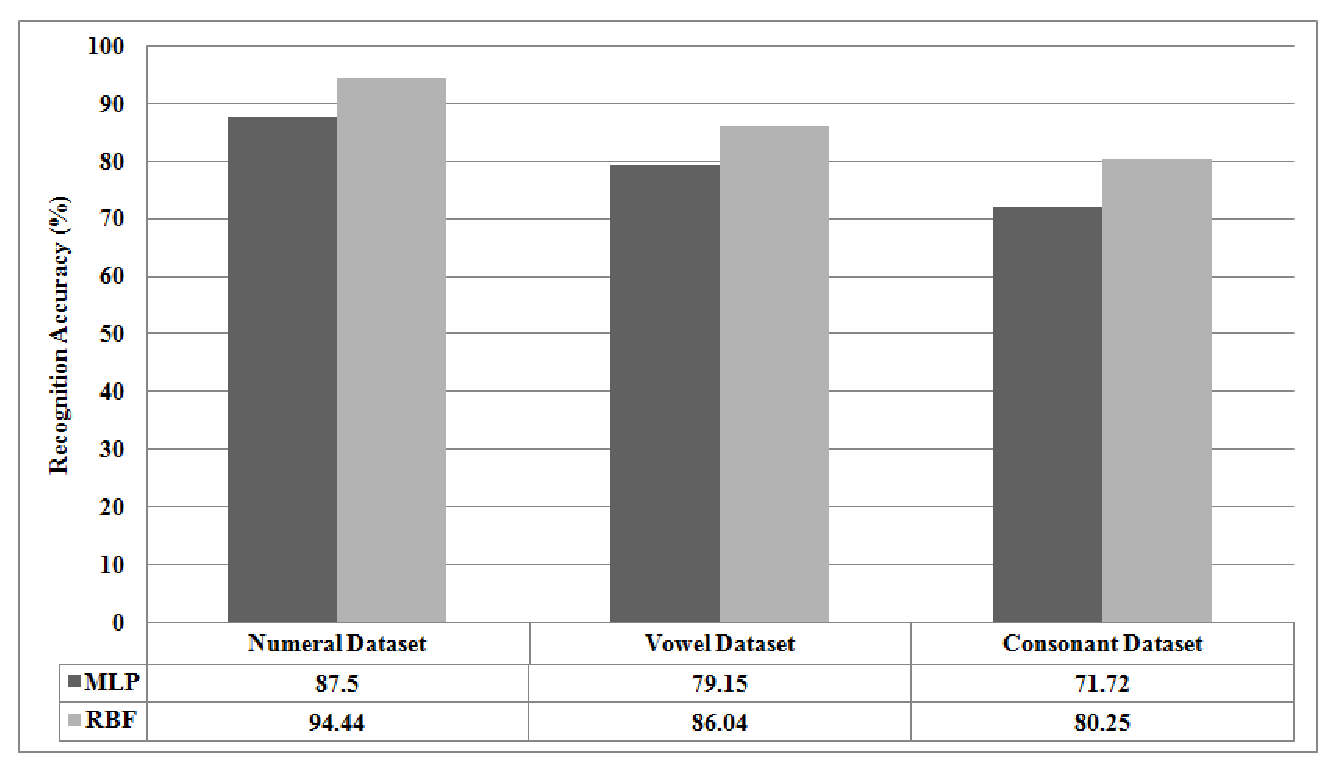
\includegraphics[scale=0.60]{figures/experiments/recognition_accuracy}
\caption{Recognition Accuracy of Off-line Handwriting Recognition Systems.}
\label{figure_recognition_accuracy_graph}
\end{figure}

Figure \ref{figure_training_time_graph} shows the graph of training time for each recognition systems in each datasets.
\begin{figure}[h]
\centering
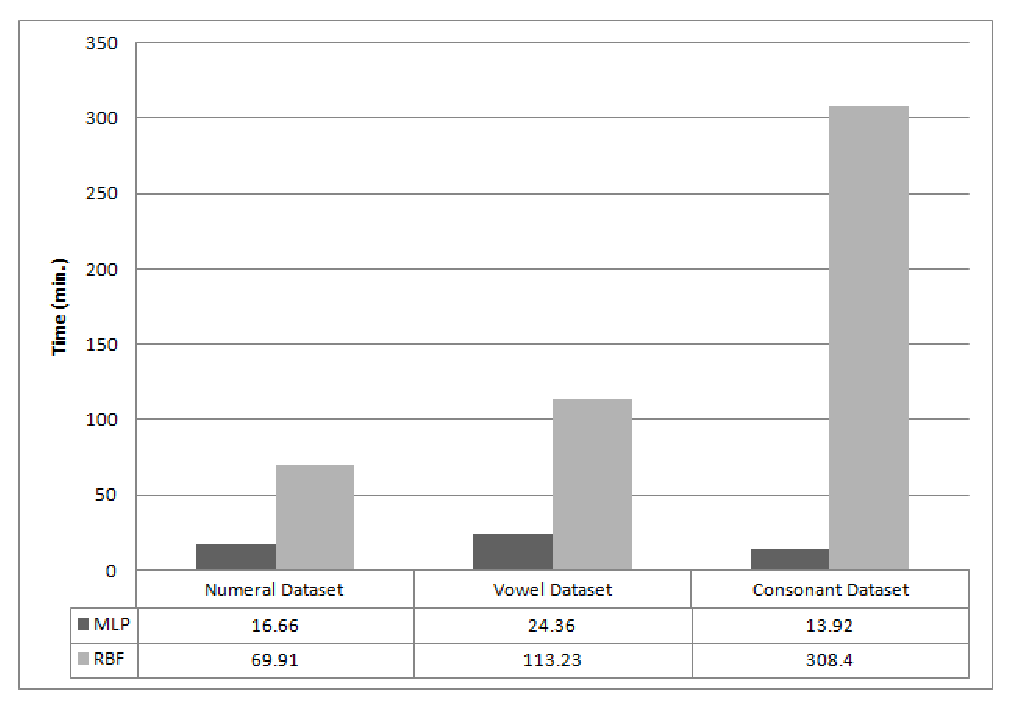
\includegraphics[scale=0.80]{figures/experiments/training_time.eps}
\caption{Training Time of Off-line Handwriting Recognition Systems.}
\label{figure_training_time_graph}
\end{figure}

\pagebreak
Table \ref{table_recognition_result_for_individual_numerals} shows individual recognition results for Nepali handwritten numeral dataset for each classes. The corresponding \ac{cm}  for test set of numeral dataset is given in table \ref{table_numeral_cm}. The numeral test set contains $576$ random samples for testing. Here, $CM$ is an $10$x$10$ matrix with $CM(i,j)$ is the number of target samples of the $i^{th}$ class classified by the outputs into class $j$.

% Recognition Results for Individual Numerals.
\begin{table}[h]
\centering
\begin{tabular}{|c|c|c|c|c|c|}
\hline
\multirow{2}{*}{\textbf{Class}} & \textbf{Recognition} & \textbf{Recognition } & \multirow{2}{*}{\textbf{Class}} & \textbf{Recognition} & \textbf{Recognition }\tabularnewline
 & \textbf{Algorithms} & \textbf{Accuracy (\%)} &  & \textbf{Algorithms} & \textbf{Accuracy (\%)}\tabularnewline
\hline
\multirow{2}{*}{
\includegraphics[scale=0.25]{figures/datasets/nhcr/numerals/zero}} & MLP & 97.7 & \multirow{2}{*}{
\includegraphics[scale=0.25]{figures/datasets/nhcr/numerals/one}} & MLP & 94.1\tabularnewline
\cline{2-3} \cline{5-6}
 & RBF & 98.6 &  & RBF & 98.4\tabularnewline
\hline
\multirow{2}{*}{
\includegraphics[scale=0.25]{figures/datasets/nhcr/numerals/two}} & MLP & 85.1 & \multirow{2}{*}{
\includegraphics[scale=0.25]{figures/datasets/nhcr/numerals/three}} & MLP & 82.1\tabularnewline
\cline{2-3} \cline{5-6}
 & RBF & 93.0 &  & RBF & 90.4\tabularnewline
\hline
\multirow{2}{*}{
\includegraphics[scale=0.25]{figures/datasets/nhcr/numerals/four}} & MLP & 82.5 & \multirow{2}{*}{
\includegraphics[scale=0.25]{figures/datasets/nhcr/numerals/five}} & MLP & 82.5\tabularnewline
\cline{2-3} \cline{5-6}
 & RBF & 98.0 &  & RBF & 81.1\tabularnewline
\hline
\multirow{2}{*}{
\includegraphics[scale=0.25]{figures/datasets/nhcr/numerals/six}} & MLP & 82.9 & \multirow{2}{*}{
\includegraphics[scale=0.25]{figures/datasets/nhcr/numerals/seven}} & MLP & 86.7\tabularnewline
\cline{2-3} \cline{5-6}
 & RBF & 95.0 &  & RBF & 96.2\tabularnewline
\hline
\multirow{2}{*}{
\includegraphics[scale=0.25]{figures/datasets/nhcr/numerals/eight}} & MLP & 97.8 & \multirow{2}{*}{
\includegraphics[scale=0.25]{figures/datasets/nhcr/numerals/nine}} & MLP & 80.4\tabularnewline
\cline{2-3} \cline{5-6}
 & RBF & 100 &  & RBF & 90.9\tabularnewline
\hline
\end{tabular}
\caption{Recognition Results For Individual Numerals.}
\label{table_recognition_result_for_individual_numerals}
\end{table}

%Confusion Matrix of Numeral Database Testing.
\begin{table}[h]
\centering
\begin{tabular}{|c|c|c|c|c|c|c|c|c|c|c|}
\hline
\textbf{Class} & 
\includegraphics[scale=0.25]{figures/datasets/nhcr/numerals/zero} & 
\includegraphics[scale=0.25]{figures/datasets/nhcr/numerals/one} & 
\includegraphics[scale=0.25]{figures/datasets/nhcr/numerals/two} & 
\includegraphics[scale=0.25]{figures/datasets/nhcr/numerals/three} & 
\includegraphics[scale=0.25]{figures/datasets/nhcr/numerals/four} & 
\includegraphics[scale=0.25]{figures/datasets/nhcr/numerals/five} & 
\includegraphics[scale=0.25]{figures/datasets/nhcr/numerals/six} & 
\includegraphics[scale=0.25]{figures/datasets/nhcr/numerals/seven} & 
\includegraphics[scale=0.25]{figures/datasets/nhcr/numerals/eight} & 
\includegraphics[scale=0.25]{figures/datasets/nhcr/numerals/nine}\tabularnewline
\hline

\includegraphics[scale=0.25]{figures/datasets/nhcr/numerals/zero} & 69 & 0 & 0 & 0 & 0 & 0 & 0 & 0 & 0 & 1\tabularnewline
\hline

\includegraphics[scale=0.25]{figures/datasets/nhcr/numerals/one} & 0 & 61 & 0 & 0 & 0 & 0 & 1 & 0 & 0 & 0\tabularnewline
\hline

\includegraphics[scale=0.25]{figures/datasets/nhcr/numerals/two} & 0 & 0 & 53 & 4 & 0 & 0 & 0 & 0 & 0 & 0\tabularnewline
\hline

\includegraphics[scale=0.25]{figures/datasets/nhcr/numerals/three} & 0 & 0 & 3 & 47 & 0 & 0 & 2 & 0 & 0 & 0\tabularnewline
\hline

\includegraphics[scale=0.25]{figures/datasets/nhcr/numerals/four} & 0 & 0 & 0 & 0 & 49 & 1 & 0 & 0 & 0 & 0\tabularnewline
\hline

\includegraphics[scale=0.25]{figures/datasets/nhcr/numerals/five} & 0 & 0 & 5 & 3 & 1 & 43 & 0 & 0 & 0 & 1\tabularnewline
\hline

\includegraphics[scale=0.25]{figures/datasets/nhcr/numerals/six} & 0 & 1 & 0 & 0 & 0 & 0 & 57 & 1 & 0 & 0\tabularnewline
\hline

\includegraphics[scale=0.25]{figures/datasets/nhcr/numerals/seven} & 0 & 0 & 0 & 0 & 1 & 0 & 1 & 51 & 0 & 0\tabularnewline
\hline

\includegraphics[scale=0.25]{figures/datasets/nhcr/numerals/eight} & 0 & 0 & 0 & 0 & 0 & 0 & 0 & 0 & 64 & 0\tabularnewline
\hline

\includegraphics[scale=0.25]{figures/datasets/nhcr/numerals/nine} & 0 & 1 & 1 & 1 & 0 & 1 & 1 & 0 & 0 & 50\tabularnewline
\hline
\end{tabular}
\caption{Confusion Matrix of Numeral Dataset Testing.}
\label{table_numeral_cm}
\end{table}

Figure \ref{figure_recognition_accuracy_numerals} shows the graph of recognition accuracy for each classes of numeral dataset.
\begin{figure}[h]
\centering
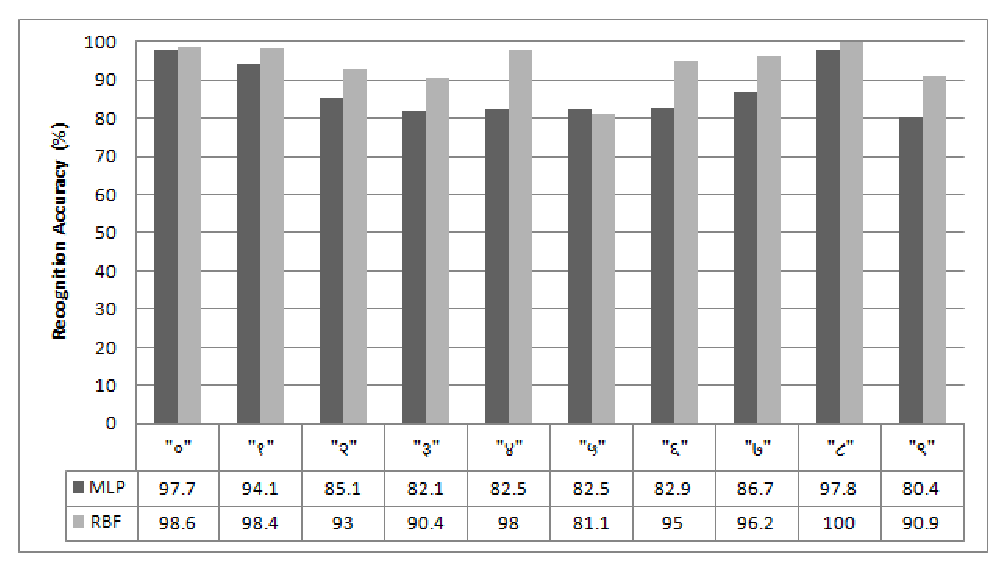
\includegraphics[scale=0.60]{figures/experiments/recognition_accuracy_numerals.eps}
\caption{Recognition Accuracy of Each Numeral Classes.}
\label{figure_recognition_accuracy_numerals}
\end{figure}

\pagebreak
Table \ref{table_recognition_result_for_individual_vowels} shows individual recognition results for Nepali handwritten vowel dataset for each classes. The corresponding \ac{cm}  for test set of vowel dataset is given in table \ref{table_vowel_cm}. The vowel test set contains $530$ random samples for testing. Here, $CM$ is an $12$x$12$ matrix with $CM(i,j)$ is the number of target samples of the $i^{th}$ class classified by the outputs into class $j$.

% Recognition Results for Individual Vowels
\begin{table}[h]
\centering
\begin{tabular}{|c|c|c|c|c|c|}
\hline
\multirow{2}{*}{\textbf{Class}} & \textbf{Recognition} & \textbf{Recognition } & \multirow{2}{*}{\textbf{Class}} & \textbf{Recognition} & \textbf{Recognition }\tabularnewline
 & \textbf{Algorithms} & \textbf{Accuracy (\%)} &  & \textbf{Algorithms} & \textbf{Accuracy (\%)}\tabularnewline
\hline
\multirow{2}{*}{
\includegraphics[scale=0.25]{figures/datasets/nhcr/vowels/1a}} & MLP & 77.8 & \multirow{2}{*}{
\includegraphics[scale=0.25]{figures/datasets/nhcr/vowels/2aa}} & MLP & 93.5\tabularnewline
\cline{2-3} \cline{5-6}
 & RBF & 78.9 &  & RBF & 87.8\tabularnewline
\hline
\multirow{2}{*}{
\includegraphics[scale=0.25]{figures/datasets/nhcr/vowels/3i}} & MLP & 84.2 & \multirow{2}{*}{
\includegraphics[scale=0.25]{figures/datasets/nhcr/vowels/4ee}} & MLP & 88.5\tabularnewline
\cline{2-3} \cline{5-6}
 & RBF & 91.1 &  & RBF & 90.5\tabularnewline
\hline
\multirow{2}{*}{
\includegraphics[scale=0.25]{figures/datasets/nhcr/vowels/5u}} & MLP & 75.8 & \multirow{2}{*}{
\includegraphics[scale=0.25]{figures/datasets/nhcr/vowels/6oo}} & MLP & 85.2\tabularnewline
\cline{2-3} \cline{5-6}
 & RBF & 92.1 &  & RBF & 87.8\tabularnewline
\hline
\multirow{2}{*}{
\includegraphics[scale=0.25]{figures/datasets/nhcr/vowels/7ye}} & MLP & 78.4 & \multirow{2}{*}{
\includegraphics[scale=0.25]{figures/datasets/nhcr/vowels/8ai}} & MLP & 82.9\tabularnewline
\cline{2-3} \cline{5-6}
 & RBF & 97.6 &  & RBF & 85.7\tabularnewline
\hline
\multirow{2}{*}{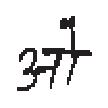
\includegraphics[scale=0.25]{figures/datasets/nhcr/vowels/9o}} & MLP & 71.4 & \multirow{2}{*}{
\includegraphics[scale=0.25]{figures/datasets/nhcr/vowels/10au}} & MLP & 64.7\tabularnewline
\cline{2-3} \cline{5-6}
 & RBF & 76.5 &  & RBF & 80.0\tabularnewline
\hline
\multirow{2}{*}{
\includegraphics[scale=0.25]{figures/datasets/nhcr/vowels/11an}} & MLP & 64.1 & \multirow{2}{*}{
\includegraphics[scale=0.25]{figures/datasets/nhcr/vowels/12ah}} & MLP & 86.5\tabularnewline
\cline{2-3} \cline{5-6}
 & RBF & 76.1 &  & RBF & 88.5\tabularnewline
\hline
\end{tabular}
\caption{Recognition Results For Individual Vowels.}
\label{table_recognition_result_for_individual_vowels}
\end{table}

%Confusion Matrix of Vowel Database Testing.
\begin{table}[h]
\centering
\begin{tabular}{|c|c|c|c|c|c|c|c|c|c|c|c|c|}
\hline
\textbf{Class} & 
\includegraphics[scale=0.25]{figures/datasets/nhcr/vowels/1a} & 
\includegraphics[scale=0.25]{figures/datasets/nhcr/vowels/2aa} & 
\includegraphics[scale=0.25]{figures/datasets/nhcr/vowels/3i} & 
\includegraphics[scale=0.25]{figures/datasets/nhcr/vowels/4ee} & 
\includegraphics[scale=0.25]{figures/datasets/nhcr/vowels/5u} & \includegraphics[scale=0.25]{figures/datasets/nhcr/vowels/6oo} & \includegraphics[scale=0.25]{figures/datasets/nhcr/vowels/7ye} & \includegraphics[scale=0.25]{figures/datasets/nhcr/vowels/8ai} & \includegraphics[scale=0.25]{figures/datasets/nhcr/vowels/9o} & \includegraphics[scale=0.25]{figures/datasets/nhcr/vowels/10au} & \includegraphics[scale=0.25]{figures/datasets/nhcr/vowels/11an} & \includegraphics[scale=0.25]{figures/datasets/nhcr/vowels/12ah}\tabularnewline
\hline
\includegraphics[scale=0.25]{figures/datasets/nhcr/vowels/1a} & 45  & 6 & 0 & 0 & 0 & 4 & 0 & 0 & 1 & 0 & 1 & 0\tabularnewline
\hline
\includegraphics[scale=0.25]{figures/datasets/nhcr/vowels/2aa} & 3 & 36 & 0 & 0 & 0 & 0 & 0 & 0 & 0 & 1 & 0 & 1\tabularnewline
\hline
\includegraphics[scale=0.25]{figures/datasets/nhcr/vowels/3i} & 0 & 0 & 51 & 0 & 1 & 0 & 0 & 0 & 1 & 1 & 2 & 0\tabularnewline
\hline
\includegraphics[scale=0.25]{figures/datasets/nhcr/vowels/4ee} & 0 & 0 & 2 & 38 & 0 & 0 & 0 & 1 & 0 & 0 & 1 & 0\tabularnewline
\hline
\includegraphics[scale=0.25]{figures/datasets/nhcr/vowels/5u} & 1 & 0 & 2 & 0 & 35 & 0 & 0 & 0 & 0 & 0 & 0 & 0\tabularnewline
\hline
\includegraphics[scale=0.25]{figures/datasets/nhcr/vowels/6oo} & 2 & 0 & 0 & 0 & 1 & 36 & 0 & 0 & 0 & 0 & 0 & 2\tabularnewline
\hline
\includegraphics[scale=0.25]{figures/datasets/nhcr/vowels/7ye} & 1 & 0 & 0 & 0 & 0 & 0 & 40 & 0 & 0 & 0 & 0 & 0\tabularnewline
\hline
\includegraphics[scale=0.25]{figures/datasets/nhcr/vowels/8ai} & 1 & 0 & 0 & 0 & 0 & 0 & 2 & 36 & 2 & 0 & 1 & 0\tabularnewline
\hline
\includegraphics[scale=0.25]{figures/datasets/nhcr/vowels/9o} & 0 & 0 & 0 & 0 & 0 & 0 & 0 & 1 & 26 & 5 & 2 & 0\tabularnewline
\hline
\includegraphics[scale=0.25]{figures/datasets/nhcr/vowels/10au} & 0 & 0 & 0 & 0 & 0 & 0 & 0 & 0 & 6 & 32 & 2 & 0\tabularnewline
\hline
\includegraphics[scale=0.25]{figures/datasets/nhcr/vowels/11an} & 1 & 0 & 0 & 2 & 0 & 0 & 0 & 1 & 5 & 2 & 35 & 0\tabularnewline
\hline
\includegraphics[scale=0.25]{figures/datasets/nhcr/vowels/12ah} & 1 & 3 & 0 & 0 & 0 & 0 & 0 & 0 & 0 & 2 & 0 & 46 \tabularnewline
\hline
\end{tabular}
\caption{Confusion Matrix of Vowel Dataset Testing.}
\label{table_vowel_cm}
\end{table}

Figure \ref{figure_recognition_accuracy_vowels} shows the graph of recognition accuracy for each classes of vowel dataset.
\begin{figure}[h]
\centering
\includegraphics[scale=0.60]{figures/experiments/recognition_accuracy_vowels.eps}
\caption{Recognition Accuracy of Each Vowel Classes.}
\label{figure_recognition_accuracy_vowels}
\end{figure}


Table \ref{table_recognition_result_for_individual_consonants} shows individual recognition results for Nepali handwritten consonant dataset for each classes. The corresponding \ac{cm}  for test set of consonant dataset is given in table \ref{table_consonant_cm1} and table \ref{table_consonant_cm2} . The consonant test set contains $891$ random samples for testing. Here, $CM$ is an $36$x$36$ matrix with $CM(i,j)$ is the number of target samples of the $j^{th}$ class classified by the outputs into class $i$.

% Recognition Results for Individual Consonants
\begin{table}[h]
\centering
\begin{tabular}{|c|c|c|c|c|c|}
\hline
\multirow{2}{*}{\textbf{Class}} & \textbf{Recognition} & \textbf{Recognition } & \multirow{2}{*}{\textbf{Class}} & \textbf{Recognition} & \textbf{Recognition }\tabularnewline
 & \textbf{Algorithms} & \textbf{Accuracy (\%)} &  & \textbf{Algorithms} & \textbf{Accuracy (\%)}\tabularnewline
\hline
\multirow{2}{*}{\includegraphics[scale=0.25]{figures/datasets/nhcr/consonants/1ka}} & MLP & 94.1 & \multirow{2}{*}{\includegraphics[scale=0.25]{figures/datasets/nhcr/consonants/2kha}} & MLP & 78.3\tabularnewline
\cline{2-3} \cline{5-6}
 & RBF & 94.1 &  & RBF & 91.3\tabularnewline
\hline
\multirow{2}{*}{\includegraphics[scale=0.25]{figures/datasets/nhcr/consonants/3ga}} & MLP & 80.8 & \multirow{2}{*}{\includegraphics[scale=0.25]{figures/datasets/nhcr/consonants/4gha}} & MLP & 51.9\tabularnewline
\cline{2-3} \cline{5-6}
 & RBF & 92.3 &  & RBF & 77.8\tabularnewline
\hline
\multirow{2}{*}{\includegraphics[scale=0.25]{figures/datasets/nhcr/consonants/5na}} & MLP & 60.0 & \multirow{2}{*}{\includegraphics[scale=0.25]{figures/datasets/nhcr/consonants/6cha}} & MLP & 84.6\tabularnewline
\cline{2-3} \cline{5-6}
 & RBF & 64.0 &  & RBF & 84.6\tabularnewline
\hline
\multirow{2}{*}{\includegraphics[scale=0.25]{figures/datasets/nhcr/consonants/7chha}} & MLP & 66.7 & \multirow{2}{*}{\includegraphics[scale=0.25]{figures/datasets/nhcr/consonants/8ja}} & MLP & 73.1\tabularnewline
\cline{2-3} \cline{5-6}
 & RBF & 77.8 &  & RBF & 80.8\tabularnewline
\hline
\multirow{2}{*}{\includegraphics[scale=0.25]{figures/datasets/nhcr/consonants/9jha}} & MLP & 65.4 & \multirow{2}{*}{\includegraphics[scale=0.25]{figures/datasets/nhcr/consonants/10yna}} & MLP & 59.4\tabularnewline
\cline{2-3} \cline{5-6}
 & RBF & 73.1 &  & RBF & 68.8\tabularnewline
\hline
\multirow{2}{*}{\includegraphics[scale=0.25]{figures/datasets/nhcr/consonants/11ta}} & MLP & 96.3 & \multirow{2}{*}{\includegraphics[scale=0.25]{figures/datasets/nhcr/consonants/12tha}} & MLP & 63.6\tabularnewline
\cline{2-3} \cline{5-6}
 & RBF & 92.6 &  & RBF & 72.7\tabularnewline
\hline
\multirow{2}{*}{\includegraphics[scale=0.25]{figures/datasets/nhcr/consonants/13da}} & MLP & 76.9 & \multirow{2}{*}{\includegraphics[scale=0.25]{figures/datasets/nhcr/consonants/14dha}} & MLP & 91.7\tabularnewline
\cline{2-3} \cline{5-6}
 & RBF & 88.5 &  & RBF & 91.7\tabularnewline
\hline
\multirow{2}{*}{\includegraphics[scale=0.25]{figures/datasets/nhcr/consonants/15yna}} & MLP & 85.0 & \multirow{2}{*}{\includegraphics[scale=0.25]{figures/datasets/nhcr/consonants/16ta}} & MLP & 92.3\tabularnewline
\cline{2-3} \cline{5-6}
 & RBF & 90.0 &  & RBF & 96.2\tabularnewline
\hline
\multirow{2}{*}{\includegraphics[scale=0.25]{figures/datasets/nhcr/consonants/17tha}} & MLP & 50.0 & \multirow{2}{*}{\includegraphics[scale=0.25]{figures/datasets/nhcr/consonants/18da}} & MLP & 64.0\tabularnewline
\cline{2-3} \cline{5-6}
 & RBF & 72.7 &  & RBF & 76.0\tabularnewline
\hline
\multirow{2}{*}{\includegraphics[scale=0.25]{figures/datasets/nhcr/consonants/19dha}} & MLP & 75.0 & \multirow{2}{*}{\includegraphics[scale=0.25]{figures/datasets/nhcr/consonants/20na}} & MLP & 36.8\tabularnewline
\cline{2-3} \cline{5-6}
 & RBF & 79.2 &  & RBF & 38.8\tabularnewline
\hline
\multirow{2}{*}{\includegraphics[scale=0.25]{figures/datasets/nhcr/consonants/21pa}} & MLP & 87.5 & \multirow{2}{*}{\includegraphics[scale=0.25]{figures/datasets/nhcr/consonants/22pha}} & MLP & 72.4\tabularnewline
\cline{2-3} \cline{5-6}
 & RBF & 100 &  & RBF & 86.2\tabularnewline
\hline
\multirow{2}{*}{\includegraphics[scale=0.25]{figures/datasets/nhcr/consonants/23ba}} & MLP & 75.9 & \multirow{2}{*}{\includegraphics[scale=0.25]{figures/datasets/nhcr/consonants/24bha}} & MLP & 63.6\tabularnewline
\cline{2-3} \cline{5-6}
 & RBF & 75.9 &  & RBF & 90.9\tabularnewline
\hline
\multirow{2}{*}{\includegraphics[scale=0.25]{figures/datasets/nhcr/consonants/25ma}} & MLP & 66.7 & \multirow{2}{*}{\includegraphics[scale=0.25]{figures/datasets/nhcr/consonants/26ya}} & MLP & 44.0\tabularnewline
\cline{2-3} \cline{5-6}
 & RBF & 73.3 &  & RBF & 56.0\tabularnewline
\hline
\multirow{2}{*}{\includegraphics[scale=0.25]{figures/datasets/nhcr/consonants/27ra}} & MLP & 89.3 & \multirow{2}{*}{\includegraphics[scale=0.25]{figures/datasets/nhcr/consonants/28la}} & MLP & 66.7\tabularnewline
\cline{2-3} \cline{5-6}
 & RBF & 82.1 &  & RBF & 77.8\tabularnewline
\hline
\multirow{2}{*}{\includegraphics[scale=0.25]{figures/datasets/nhcr/consonants/29wa}} & MLP & 73.9 & \multirow{2}{*}{\includegraphics[scale=0.25]{figures/datasets/nhcr/consonants/30sa}} & MLP & 80.0\tabularnewline
\cline{2-3} \cline{5-6}
 & RBF & 78.3 &  & RBF & 91.4\tabularnewline
\hline
\multirow{2}{*}{\includegraphics[scale=0.25]{figures/datasets/nhcr/consonants/31khasa}} & MLP & 76.0 & \multirow{2}{*}{\includegraphics[scale=0.25]{figures/datasets/nhcr/consonants/32saa}} & MLP & 55.2\tabularnewline
\cline{2-3} \cline{5-6}
 & RBF & 80.0 &  & RBF & 79.3\tabularnewline
\hline
\multirow{2}{*}{\includegraphics[scale=0.25]{figures/datasets/nhcr/consonants/33ha}} & MLP & 88.2 & \multirow{2}{*}{\includegraphics[scale=0.25]{figures/datasets/nhcr/consonants/34kchya}} & MLP & 60.0\tabularnewline
\cline{2-3} \cline{5-6}
 & RBF & 82.4 &  & RBF & 72.0\tabularnewline
\hline
\multirow{2}{*}{\includegraphics[scale=0.25]{figures/datasets/nhcr/consonants/35tra}} & MLP & 73.1 & \multirow{2}{*}{\includegraphics[scale=0.25]{figures/datasets/nhcr/consonants/36gya}} & MLP & 64.0\tabularnewline
\cline{2-3} \cline{5-6}
 & RBF & 76.9 &  & RBF & 80.0\tabularnewline
\hline
\end{tabular}
\caption{Recognition Results For Individual Characters.}
\label{table_recognition_result_for_individual_consonants}
\end{table}

%Confusion Matrix 1 of Consonant Database Testing.
\begin{table}[h]
\centering
\begin{tabular}{|c|c|c|c|c|c|c|c|c|c|c|c|c|c|c|c|c|c|c|}
\hline
\textbf{Class} & \includegraphics[scale=0.25]{figures/datasets/nhcr/consonants/1ka} & \includegraphics[scale=0.25]{figures/datasets/nhcr/consonants/2kha} & \includegraphics[scale=0.25]{figures/datasets/nhcr/consonants/3ga} & \includegraphics[scale=0.25]{figures/datasets/nhcr/consonants/4gha} & \includegraphics[scale=0.25]{figures/datasets/nhcr/consonants/5na} & \includegraphics[scale=0.25]{figures/datasets/nhcr/consonants/6cha} & \includegraphics[scale=0.25]{figures/datasets/nhcr/consonants/7chha} & \includegraphics[scale=0.25]{figures/datasets/nhcr/consonants/8ja} & \includegraphics[scale=0.25]{figures/datasets/nhcr/consonants/9jha} & \includegraphics[scale=0.25]{figures/datasets/nhcr/consonants/10yna} & \includegraphics[scale=0.25]{figures/datasets/nhcr/consonants/11ta} & \includegraphics[scale=0.25]{figures/datasets/nhcr/consonants/12tha} & \includegraphics[scale=0.25]{figures/datasets/nhcr/consonants/13da} & \includegraphics[scale=0.25]{figures/datasets/nhcr/consonants/14dha} & \includegraphics[scale=0.25]{figures/datasets/nhcr/consonants/15yna} & \includegraphics[scale=0.25]{figures/datasets/nhcr/consonants/16ta} & \includegraphics[scale=0.25]{figures/datasets/nhcr/consonants/17tha} & \includegraphics[scale=0.25]{figures/datasets/nhcr/consonants/18da}\tabularnewline
\hline
\includegraphics[scale=0.25]{figures/datasets/nhcr/consonants/1ka} & 16 & 0 & 0 & 0 & 1 & 0 & 0 & 0 & 1 & 0 & 0 & 0 & 0 & 0 & 0 & 0 & 0 & 1\tabularnewline
\hline
\includegraphics[scale=0.25]{figures/datasets/nhcr/consonants/2kha} & 0 & 21 & 0 & 0 & 0 & 0 & 0 & 0 & 1 & 0 & 0 & 0 & 0 & 1 & 0 & 0 & 0 & 0\tabularnewline
\hline
\includegraphics[scale=0.25]{figures/datasets/nhcr/consonants/3ga} & 0 & 0 & 24 & 0 & 0 & 0 & 0 & 0 & 0 & 1 & 0 & 0 & 0 & 0 & 1 & 0 & 0 & 0\tabularnewline
\hline
\includegraphics[scale=0.25]{figures/datasets/nhcr/consonants/4gha} & 0 & 0 & 0 & 21 & 0 & 1 & 0 & 0 & 0 & 0 & 0 & 0 & 0 & 0 & 0 & 0 & 1 & 0\tabularnewline
\hline
\includegraphics[scale=0.25]{figures/datasets/nhcr/consonants/5na} & 0 & 0 & 0 & 0 & 16 & 0 & 0 & 0 & 0 & 0 & 0 & 0 & 1 & 0 & 0 & 0 & 0 & 0\tabularnewline
\hline
\includegraphics[scale=0.25]{figures/datasets/nhcr/consonants/6cha} & 0 & 0 & 0 & 0 & 0 & 22 & 0 & 0 & 0 & 0 & 0 & 0 & 0 & 0 & 0 & 0 & 0 & 0\tabularnewline
\hline
\includegraphics[scale=0.25]{figures/datasets/nhcr/consonants/7chha} & 0 & 0 & 0 & 1 & 0 & 0 & 14 & 0 & 0 & 0 & 1 & 0 & 0 & 0 & 0 & 0 & 0 & 2\tabularnewline
\hline
\includegraphics[scale=0.25]{figures/datasets/nhcr/consonants/8ja} & 0 & 0 & 0 & 0 & 1 & 0 & 0 & 21 & 0 & 1 & 0 & 0 & 0 & 0 & 0 & 0 & 0 & 0\tabularnewline
\hline
\includegraphics[scale=0.25]{figures/datasets/nhcr/consonants/9jha} & 0 & 0 & 0 & 0 & 0 & 0 & 1 & 0 & 19 & 0 & 0 & 0 & 0 & 0 & 0 & 0 & 0 & 0\tabularnewline
\hline
\includegraphics[scale=0.25]{figures/datasets/nhcr/consonants/10yna} & 0 & 0 & 0 & 0 & 0 & 0 & 0 & 3 & 0 & 22 & 0 & 0 & 0 & 0 & 0 & 0 & 0 & 0\tabularnewline
\hline
\includegraphics[scale=0.25]{figures/datasets/nhcr/consonants/11ta} & 0 & 0 & 0 & 0 & 0 & 0 & 0 & 0 & 0 & 0 & 25 & 0 & 0 & 0 & 0 & 0 & 0 & 0\tabularnewline
\hline
\includegraphics[scale=0.25]{figures/datasets/nhcr/consonants/12tha} & 0 & 0 & 0 & 0 & 0 & 0 & 0 & 0 & 0 & 0 & 0 & 16 & 0 & 0 & 0 & 0 & 0 & 1\tabularnewline
\hline
\includegraphics[scale=0.25]{figures/datasets/nhcr/consonants/13da} & 0 & 0 & 0 & 0 & 2 & 0 & 0 & 0 & 0 & 0 & 0 & 1 & 23 & 1 & 0 & 0 & 0 & 0\tabularnewline
\hline
\includegraphics[scale=0.25]{figures/datasets/nhcr/consonants/14dha} & 0 & 0 & 0 & 0 & 1 & 0 & 1 & 0 & 0 & 0 & 0 & 1 & 0 & 22 & 0 & 0 & 0 & 1\tabularnewline
\hline
\includegraphics[scale=0.25]{figures/datasets/nhcr/consonants/15yna} & 0 & 0 & 0 & 0 & 0 & 0 & 0 & 0 & 0 & 0 & 0 & 0 & 0 & 0 & 18 & 0 & 0 & 0\tabularnewline
\hline
\includegraphics[scale=0.25]{figures/datasets/nhcr/consonants/16ta} & 0 & 0 & 0 & 0 & 0 & 0 & 0 & 0 & 0 & 0 & 0 & 0 & 0 & 0 & 0 & 25 & 0 & 0\tabularnewline
\hline
\includegraphics[scale=0.25]{figures/datasets/nhcr/consonants/17tha} & 0 & 0 & 0 & 1 & 0 & 0 & 0 & 0 & 0 & 0 & 0 & 0 & 0 & 0 & 0 & 0 & 16 & 0\tabularnewline
\hline
\includegraphics[scale=0.25]{figures/datasets/nhcr/consonants/18da} & 0 & 0 & 0 & 0 & 1 & 0 & 0 & 0 & 0 & 0 & 0 & 2 & 0 & 0 & 0 & 0 & 0 & 19\tabularnewline
\hline
\includegraphics[scale=0.25]{figures/datasets/nhcr/consonants/19dha} & 0 & 0 & 0 & 1 & 0 & 1 & 0 & 0 & 0 & 0 & 0 & 1 & 0 & 0 & 1 & 0 & 2 & 0\tabularnewline
\hline
\includegraphics[scale=0.25]{figures/datasets/nhcr/consonants/20na} & 0 & 0 & 0 & 0 & 0 & 0 & 0 & 0 & 0 & 0 & 0 & 0 & 0 & 0 & 0 & 0 & 0 & 0\tabularnewline
\hline
\includegraphics[scale=0.25]{figures/datasets/nhcr/consonants/21pa} & 0 & 0 & 0 & 2 & 0 & 0 & 0 & 0 & 0 & 0 & 0 & 0 & 0 & 0 & 0 & 1 & 1 & 0\tabularnewline
\hline
\includegraphics[scale=0.25]{figures/datasets/nhcr/consonants/22pha} & 0 & 0 & 0 & 0 & 0 & 0 & 0 & 0 & 1 & 0 & 0 & 0 & 0 & 0 & 0 & 0 & 0 & 0\tabularnewline
\hline
\includegraphics[scale=0.25]{figures/datasets/nhcr/consonants/23ba} & 0 & 0 & 0 & 0 & 0 & 0 & 0 & 0 & 0 & 2 & 0 & 0 & 0 & 0 & 0 & 0 & 1 & 0\tabularnewline
\hline
\includegraphics[scale=0.25]{figures/datasets/nhcr/consonants/24bha} & 0 & 0 & 0 & 0 & 0 & 0 & 0 & 0 & 0 & 1 & 0 & 0 & 0 & 0 & 0 & 0 & 0 & 0\tabularnewline
\hline
\includegraphics[scale=0.25]{figures/datasets/nhcr/consonants/25ma} & 0 & 0 & 1 & 0 & 0 & 0 & 0 & 0 & 0 & 2 & 0 & 1 & 0 & 0 & 0 & 0 & 0 & 0\tabularnewline
\hline
\includegraphics[scale=0.25]{figures/datasets/nhcr/consonants/26ya} & 0 & 0 & 0 & 0 & 0 & 1 & 0 & 0 & 0 & 0 & 0 & 0 & 0 & 0 & 0 & 0 & 1 & 1\tabularnewline
\hline
\includegraphics[scale=0.25]{figures/datasets/nhcr/consonants/27ra} & 0 & 0 & 0 & 0 & 0 & 0 & 0 & 0 & 0 & 0 & 0 & 0 & 1 & 0 & 0 & 0 & 0 & 0\tabularnewline
\hline
\includegraphics[scale=0.25]{figures/datasets/nhcr/consonants/28la} & 0 & 0 & 0 & 0 & 0 & 0 & 0 & 0 & 0 & 0 & 0 & 0 & 0 & 0 & 0 & 0 & 0 & 0\tabularnewline
\hline
\includegraphics[scale=0.25]{figures/datasets/nhcr/consonants/29wa} & 0 & 0 & 0 & 1 & 1 & 1 & 0 & 0 & 0 & 0 & 0 & 0 & 1 & 0 & 0 & 0 & 0 & 0\tabularnewline
\hline
\includegraphics[scale=0.25]{figures/datasets/nhcr/consonants/30sa} & 0 & 0 & 1 & 0 & 2 & 0 & 0 & 0 & 1 & 0 & 0 & 0 & 0 & 0 & 0 & 0 & 0 & 0\tabularnewline
\hline
\includegraphics[scale=0.25]{figures/datasets/nhcr/consonants/31khasa} & 1 & 0 & 0 & 0 & 0 & 0 & 0 & 0 & 0 & 0 & 0 & 0 & 0 & 0 & 0 & 0 & 0 & 0\tabularnewline
\hline
\includegraphics[scale=0.25]{figures/datasets/nhcr/consonants/32saa} & 0 & 1 & 0 & 0 & 0 & 0 & 1 & 0 & 1 & 0 & 0 & 0 & 0 & 0 & 0 & 0 & 0 & 0\tabularnewline
\hline
\includegraphics[scale=0.25]{figures/datasets/nhcr/consonants/33ha} & 0 & 0 & 0 & 0 & 0 & 0 & 1 & 0 & 0 & 0 & 1 & 0 & 0 & 0 & 0 & 0 & 0 & 0\tabularnewline
\hline
\includegraphics[scale=0.25]{figures/datasets/nhcr/consonants/34kchya} & 0 & 1 & 0 & 0 & 0 & 0 & 0 & 0 & 1 & 0 & 0 & 0 & 0 & 0 & 0 & 0 & 0 & 0\tabularnewline
\hline
\includegraphics[scale=0.25]{figures/datasets/nhcr/consonants/35tra} & 0 & 0 & 0 & 0 & 0 & 0 & 0 & 1 & 0 & 3 & 0 & 0 & 0 & 0 & 0 & 0 & 0 & 0\tabularnewline
\hline
\includegraphics[scale=0.25]{figures/datasets/nhcr/consonants/36gya} & 0 & 0 & 0 & 0 & 0 & 0 & 0 & 1 & 1 & 0 & 0 & 0 & 0 & 0 & 0 & 0 & 0 & 0\tabularnewline
\hline
\end{tabular}
\caption{Confusion Matrix (I) of Consonant Dataset Testing.}
\label{table_consonant_cm1}
\end{table}

%Confusion Matrix 2 of Consonant Database Testing.
\begin{table}[h]
\centering
\begin{tabular}{|c|c|c|c|c|c|c|c|c|c|c|c|c|c|c|c|c|c|c|}
\hline
\textbf{Class} & \includegraphics[scale=0.25]{figures/datasets/nhcr/consonants/19dha} & \includegraphics[scale=0.25]{figures/datasets/nhcr/consonants/20na} & \includegraphics[scale=0.25]{figures/datasets/nhcr/consonants/21pa} & \includegraphics[scale=0.25]{figures/datasets/nhcr/consonants/22pha} & \includegraphics[scale=0.25]{figures/datasets/nhcr/consonants/23ba} & \includegraphics[scale=0.25]{figures/datasets/nhcr/consonants/24bha} & \includegraphics[scale=0.25]{figures/datasets/nhcr/consonants/25ma} & \includegraphics[scale=0.25]{figures/datasets/nhcr/consonants/26ya} & \includegraphics[scale=0.25]{figures/datasets/nhcr/consonants/27ra} & \includegraphics[scale=0.25]{figures/datasets/nhcr/consonants/28la} & \includegraphics[scale=0.25]{figures/datasets/nhcr/consonants/29wa} & \includegraphics[scale=0.25]{figures/datasets/nhcr/consonants/30sa} & \includegraphics[scale=0.25]{figures/datasets/nhcr/consonants/31khasa} & \includegraphics[scale=0.25]{figures/datasets/nhcr/consonants/32saa} & \includegraphics[scale=0.25]{figures/datasets/nhcr/consonants/33ha} & \includegraphics[scale=0.25]{figures/datasets/nhcr/consonants/34kchya} & \includegraphics[scale=0.25]{figures/datasets/nhcr/consonants/35tra}  & \includegraphics[scale=0.25]{figures/datasets/nhcr/consonants/36gya}\tabularnewline
\hline
\includegraphics[scale=0.25]{figures/datasets/nhcr/consonants/1ka} & 0 & 0 & 0 & 0 & 1 & 0 & 0 & 0 & 0 & 0 & 0 & 0 & 0 & 0 & 0 & 0 & 1 & 0\tabularnewline
\hline
\includegraphics[scale=0.25]{figures/datasets/nhcr/consonants/2kha} & 0 & 0 & 0 & 0 & 0 & 0 & 0 & 0 & 0 & 0 & 0 & 0 & 0 & 0 & 0 & 0 & 0 & 0\tabularnewline
\hline
\includegraphics[scale=0.25]{figures/datasets/nhcr/consonants/3ga} & 0 & 1 & 0 & 0 & 0 & 0 & 0 & 1 & 0 & 0 & 0 & 0 & 0 & 0 & 0 & 1 & 2 & 0\tabularnewline
\hline
\includegraphics[scale=0.25]{figures/datasets/nhcr/consonants/4gha} & 1 & 0 & 0 & 0 & 0 & 0 & 0 & 0 & 0 & 0 & 0 & 0 & 0 & 0 & 0 & 0 & 0 & 0\tabularnewline
\hline
\includegraphics[scale=0.25]{figures/datasets/nhcr/consonants/5na} & 0 & 0 & 0 & 0 & 0 & 0 & 0 & 0 & 0 & 0 & 0 & 0 & 0 & 0 & 0 & 0 & 0 & 0\tabularnewline
\hline
\includegraphics[scale=0.25]{figures/datasets/nhcr/consonants/6cha} & 1 & 0 & 0 & 0 & 0 & 0 & 0 & 1 & 1 & 0 & 0 & 0 & 0 & 0 & 0 & 0 & 1 & 0\tabularnewline
\hline
\includegraphics[scale=0.25]{figures/datasets/nhcr/consonants/7chha} & 0 & 0 & 0 & 0 & 0 & 0 & 0 & 0 & 0 & 0 & 0 & 0 & 2 & 0 & 0 & 0 & 0 & 0\tabularnewline
\hline
\includegraphics[scale=0.25]{figures/datasets/nhcr/consonants/8ja} & 0 & 1 & 0 & 0 & 0 & 0 & 2 & 1 & 0 & 0 & 0 & 0 & 0 & 0 & 0 & 0 & 2 & 0\tabularnewline
\hline
\includegraphics[scale=0.25]{figures/datasets/nhcr/consonants/9jha} & 0 & 0 & 0 & 2 & 0 & 0 & 0 & 0 & 0 & 0 & 0 & 0 & 0 & 0 & 0 & 0 & 0 & 0\tabularnewline
\hline
\includegraphics[scale=0.25]{figures/datasets/nhcr/consonants/10yna} & 0 & 2 & 0 & 0 & 0 & 1 & 1 & 0 & 0 & 0 & 0 & 0 & 0 & 0 & 0 & 1 & 0 & 0\tabularnewline
\hline
\includegraphics[scale=0.25]{figures/datasets/nhcr/consonants/11ta} & 0 & 0 & 0 & 0 & 0 & 0 & 0 & 0 & 1 & 0 & 0 & 0 & 0 & 0 & 0 & 0 & 0 & 0\tabularnewline
\hline
\includegraphics[scale=0.25]{figures/datasets/nhcr/consonants/12tha} & 0 & 0 & 0 & 0 & 1 & 0 & 0 & 0 & 0 & 1 & 0 & 0 & 0 & 0 & 0 & 0 & 0 & 0\tabularnewline
\hline
\includegraphics[scale=0.25]{figures/datasets/nhcr/consonants/13da} & 0 & 0 & 0 & 0 & 0 & 0 & 0 & 0 & 0 & 0 & 0 & 0 & 0 & 0 & 0 & 0 & 0 & 0\tabularnewline
\hline
\includegraphics[scale=0.25]{figures/datasets/nhcr/consonants/14dha} & 0 & 0 & 0 & 0 & 0 & 0 & 1 & 0 & 0 & 0 & 0 & 0 & 0 & 0 & 1 & 0 & 0 & 0\tabularnewline
\hline
\includegraphics[scale=0.25]{figures/datasets/nhcr/consonants/15yna} & 0 & 0 & 0 & 1 & 0 & 0 & 0 & 2 & 0 & 1 & 1 & 0 & 1 & 0 & 0 & 0 & 0 & 0\tabularnewline
\hline
\includegraphics[scale=0.25]{figures/datasets/nhcr/consonants/16ta} & 0 & 2 & 0 & 0 & 0 & 0 & 0 & 1 & 1 & 1 & 0 & 0 & 0 & 0 & 0 & 0 & 0 & 0\tabularnewline
\hline
\includegraphics[scale=0.25]{figures/datasets/nhcr/consonants/17tha} & 1 & 0 & 0 & 0 & 1 & 0 & 0 & 0 & 1 & 0 & 0 & 1 & 2 & 0 & 0 & 1 & 0 & 1\tabularnewline
\hline
\includegraphics[scale=0.25]{figures/datasets/nhcr/consonants/18da} & 0 & 0 & 0 & 0 & 2 & 0 & 0 & 0 & 0 & 0 & 1 & 0 & 0 & 0 & 0 & 0 & 0 & 0\tabularnewline
\hline
\includegraphics[scale=0.25]{figures/datasets/nhcr/consonants/19dha} & 19 & 0 & 0 & 0 & 0 & 0 & 0 & 0 & 0 & 0 & 0 & 0 & 0 & 0 & 0 & 0 & 0 & 0\tabularnewline
\hline
\includegraphics[scale=0.25]{figures/datasets/nhcr/consonants/20na} & 0 & 7 & 0 & 0 & 0 & 0 & 0 & 0 & 0 & 0 & 0 & 0 & 0 & 0 & 0 & 1 & 0 & 0\tabularnewline
\hline
\includegraphics[scale=0.25]{figures/datasets/nhcr/consonants/21pa} & 0 & 0 & 24 & 1 & 0 & 1 & 2 & 3 & 0 & 0 & 0 & 0 & 0 & 0 & 1 & 0 & 0 & 0\tabularnewline
\hline
\includegraphics[scale=0.25]{figures/datasets/nhcr/consonants/22pha} & 0 & 0 & 0 & 25 & 0 & 0 & 0 & 0 & 0 & 0 & 0 & 0 & 0 & 0 & 0 & 0 & 0 & 0\tabularnewline
\hline
\includegraphics[scale=0.25]{figures/datasets/nhcr/consonants/23ba} & 0 & 0 & 0 & 0 & 22 & 0 & 0 & 0 & 0 & 0 & 1 & 1 & 0 & 0 & 0 & 1 & 0 & 1\tabularnewline
\hline
\includegraphics[scale=0.25]{figures/datasets/nhcr/consonants/24bha} & 1 & 0 & 0 & 0 & 0 & 20 & 0 & 1 & 0 & 0 & 0 & 0 & 0 & 1 & 0 & 1 & 0 & 0\tabularnewline
\hline
\includegraphics[scale=0.25]{figures/datasets/nhcr/consonants/25ma} & 0 & 2 & 0 & 0 & 1 & 0 & 22 & 0 & 0 & 0 & 0 & 0 & 0 & 2 & 0 & 0 & 0 & 0\tabularnewline
\hline
\includegraphics[scale=0.25]{figures/datasets/nhcr/consonants/26ya} & 0 & 0 & 0 & 0 & 0 & 0 & 0 & 14 & 0 & 0 & 0 & 0 & 0 & 0 & 0 & 0 & 0 & 0\tabularnewline
\hline
\includegraphics[scale=0.25]{figures/datasets/nhcr/consonants/27ra} & 0 & 1 & 0 & 0 & 0 & 0 & 0 & 0 & 23 & 0 & 0 & 0 & 0 & 0 & 0 & 0 & 0 & 0\tabularnewline
\hline
\includegraphics[scale=0.25]{figures/datasets/nhcr/consonants/28la} & 0 & 1 & 0 & 0 & 0 & 0 & 0 & 1 & 0 & 14 & 0 & 0 & 0 & 0 & 0 & 0 & 0 & 2\tabularnewline
\hline
\includegraphics[scale=0.25]{figures/datasets/nhcr/consonants/29wa} & 0 & 1 & 0 & 0 & 1 & 0 & 0 & 0 & 0 & 0 & 18 & 1 & 0 & 0 & 0 & 0 & 0 & 0\tabularnewline
\hline
\includegraphics[scale=0.25]{figures/datasets/nhcr/consonants/30sa} & 1 & 0 & 0 & 0 & 0 & 0 & 0 & 0 & 0 & 0 & 0 & 32 & 0 & 2 & 0 & 0 & 0 & 0\tabularnewline
\hline
\includegraphics[scale=0.25]{figures/datasets/nhcr/consonants/31khasa} & 0 & 0 & 0 & 0 & 0 & 0 & 0 & 0 & 0 & 0 & 0 & 0 & 20 & 0 & 1 & 0 & 0 & 0\tabularnewline
\hline
\includegraphics[scale=0.25]{figures/datasets/nhcr/consonants/32saa} & 0 & 0 & 0 & 0 & 0 & 0 & 0 & 0 & 0 & 0 & 0 & 0 & 0 & 23 & 0 & 1 & 0 & 0\tabularnewline
\hline
\includegraphics[scale=0.25]{figures/datasets/nhcr/consonants/33ha} & 0 & 0 & 0 & 0 & 0 & 0 & 0 & 0 & 0 & 0 & 1 & 0 & 0 & 0 & 14 & 0 & 0 & 0\tabularnewline
\hline
\includegraphics[scale=0.25]{figures/datasets/nhcr/consonants/34kchya} & 0 & 0 & 0 & 0 & 0 & 0 & 0 & 0 & 0 & 0 & 1 & 0 & 0 & 1 & 0 & 18 & 0 & 0\tabularnewline
\hline
\includegraphics[scale=0.25]{figures/datasets/nhcr/consonants/35tra} & 0 & 0 & 0 & 0 & 0 & 0 & 2 & 0 & 1 & 0 & 0 & 0 & 0 & 0 & 0 & 0 & 20 & 1\tabularnewline
\hline
\includegraphics[scale=0.25]{figures/datasets/nhcr/consonants/36gya} & 0 & 1 & 0 & 0 & 0 & 0 & 0 & 0 & 0 & 1 & 0 & 0 & 0 & 0 & 0 & 0 & 0 & 20\tabularnewline
\hline
\end{tabular}
\caption{Confusion Matrix (II) of Consonant Dataset Testing.}
\label{table_consonant_cm2}
\end{table}

Figure \ref{figure_recognition_accuracy_consonants} shows the graph of recognition accuracy for each classes of consonant dataset.
\begin{figure}[h]
\centering
\includegraphics[scale=0.60]{figures/experiments/recognition_accuracy_consonants11.eps}
\caption{Recognition Accuracy of Each Consonant Classes.}
\label{figure_recognition_accuracy_consonants}
\end{figure}


% see: 2Recognition of Off-Line Handwritten Devnagari Characters Using Quadratic Classifier
